\documentclass[]{article}
\usepackage{amsmath}
\usepackage{amsfonts}
\usepackage{amssymb}
\usepackage{graphicx}
\graphicspath{ {images/} }
\usepackage{fancyhdr}
\usepackage[a4paper]{geometry}
\geometry{top=2.5cm, bottom=2cm, left=2.5cm, right=2.25cm}

\providecommand{\abs}[1]{\lvert#1\rvert}
\providecommand{\norm}[1]{\lVert#1\rVert}

%opening


\begin{document}

	\begin{center}
		\textbf{{\LARGE Tema 1}}
	\end{center}
	\vspace{0.5 cm}
	
	\section{Conceptos}
	
	\begin{itemize}
		\item \textbf{Fenómenos determinísticos. }Aquellos que dan lugar al mismo resultado siempre que se realicen bajo idénticas condiciones.
		\item \textbf{Fenómenos aleatorios. }Se caracterizan porque sus resultados puede variar, incluso si el experimento se realiza bajo idénticas condiciones iniciales.
		\item \textbf{Población, colectivo o universo. }Conjunto de unidades o elementos con alguna/s característica/s en común, sobre el que se desea obtener cierta información.
		\item \textbf{Muestra.} Subconjunto de la población elegido en términos de representatividad.
		\item \textbf{Carácter o característica estadística. }Toda propiedad que se desee estudiar en la población, que debe poder observarse sobre todos y cada uno de los individuos que la componen.
			\begin{itemize}
				\item \textbf{Modalidad. }Formas posibles en las que se puede manifestar el carácter, y cada individuo o unidad de la población debe presentar una y solo una de ellas.
				\item \textbf{Carácter cualitativo (atributo). }Aquel cuyas modalidades no son medibles o cuantificables por números.
				\item \textbf{Carácter cuantitativo. }Aquel cuyas modalidades son numéricamente medibles o cuantificables.
			\end{itemize}
		\item \textbf{Escalas de medida. }La realización de cualquier estudio estadístico requiere, como primer paso, la identificación precisa de las modalidades del carácter bajo estudio y la asignación de símbolos o números a las distintas modalidades; esto es lo que se denomina \textit{medición del carácter}.
		
		Si denotamos por $X$ al carácter, y $A$ y $B$ son dos individuos cuyas medidas de $X$ son $x_A$ y $x_B$, se distinguen cuatro tipos de escala:
		\begin{itemize}
			\item \textbf{Escala nominal. }Solo se puede decir que $x_A = x_B$ o que $x_A \neq x_B$.
			\item \textbf{Escala ordinal. }No solo se puede decir que $x_A = x_B$ o $x_A \neq x_B$, sino que $x_A < x_B$ o $x_A > x_B$.
			\item \textbf{Escala de intervalo. } Se puede decir que $x_A = x_B$, $x_A \neq x_B$, $x_A < x_B$, $x_A > x_B$ y que $A$ es $x_A - x_B$ unidades diferente (superior o inferior) que $B$.
			\item \textbf{Escala de razón. }Se puede decir que $A$ es $x_A/x_B$ veces superior a $B$.
		\end{itemize}
		\item \textbf{Variable. }Una variable es un símbolo que representa a distintos valores numéricos. Cuando estos valores son el resultado de mediciones y observaciones estadística, hablaremos de variable estadística.
		
		Así, un carácter cuantitativo irá representado por una variable estadística, y sus diversas modalidades serán los valores que toma dicha variable.
		\begin{itemize}
			\item \textbf{Variables discretas. }El paso de un valor de la variable al siguiente representa un salto (el conjunto de números reales que soporta la variable está formado por puntos aislados).
			\item \textbf{Variables continuas. }La variable puede tomar todos los valores comprendidos en un intervalo de la recta real.
		\end{itemize}
	\end{itemize}

	\newpage
	
	\section{Definiciones y fórmulas}
	\begin{itemize}
		\item \underline{Frecuencia absoluta}: número total de individuos en la población que presenta dicho valor (modalidad), \textbf{$n_i$}.
		\item \underline{Frecuencia relativa}: p roporción del número de individuos que presenta  dicha modalidad, $f_i = \dfrac{n_i}{n}, ~ i = 1, \dots, k$
		$$\sum_{i = 1}^{k} n_i = n; \quad \sum_{i = 1}^{k} f_i = 1$$
		\item \underline{Frecuencia absoluta acumulada}: número de individuos que presentan un valor (modalidad) menor o igual que $x_i$
		$$N_i = \sum_{j = 1}^i n_j, i = 1, \dots, k$$
		\item \underline{Frecuencia relativa acumulada}: proporción de individuos que presentan un valor (modalidad) menor o igual que $x_i$.
		$$F_i = \dfrac{N_i}{n} = \sum_{j = 1}^i f_j, i = 1, \dots, k$$
		\item \underline{Distribución de frecuencias}: conjunto formado por cada uno de los valores (modalidades) junto con sus frecuencias
		$$\{(x_i, n_i) : i = 1, \dots, k\}$$
	\end{itemize}

	\section{Tablas estadísticas}
	
	\subsection{Variables discretas y atributos}
	
	\begin{table}[h]
		\begin{center}
			\begin{tabular}{| c | c | c | c | c |}
				\hline
				Modalidades & Frec. Abs & Frec. Rel. & Frec. Abs. Acum. & Frec. Rel. Acum. \\ \hline
				$x_1$ & $n_1$ & $f_1$ & $N_1 = n_1$ & $F_1 = f_1$ \\
				$x_2$ & $n_2$ & $f_2$ & $N_2 = n_1 + n_2$ & $F_2 = f_1 + f_2$ \\
				$\vdots$ & $\vdots$ & $\vdots$ & $\vdots$ & $\vdots$ \\
				$x_i$ & $n_i$ & $f_i$ & $N_i = n_1 + n_2 + \cdots + n_i$ & $F_i = f_1 + f_2 + \cdots + f_i$ \\
				$\vdots$ & $\vdots$ & $\vdots$ & $\vdots$ & $\vdots$ \\
				$x_k$ & $n_k$ & $f_k$ & $N_k = n_1 + n_2 + \cdots + n_k = n$ & $F_k = f_1 + f_2 + \cdots + f_k = 1$ \\
				\hline
			\end{tabular}
		\end{center}
	\end{table}

	\subsection{Variables continuas}
	
	\begin{table}[h]
		\begin{center}
			\begin{tabular}{| c | c | c | c | c | c |}
				\hline
				Intervalos & Marcas & Amplitud & Frec. Abs. & Frec. Rel. & Frec. Acum. \\ \hline
				$(e_0, e_1]$ & $c_1 = \frac{e_0 + e_1}{2}$ & $a_1 = e_1 - e_0$ & $n_1$ & $f_1$ & $N_1 = n_1$ \\
				$(e_1, e_2]$ & $c_2 = \frac{e_1 + e_2}{2}$ & $a_2 = e_2 - e_1$ & $n_2$ & $f_2$ & $N_2 = n_1 + n_2$ \\
				$\vdots$ & $\vdots$ & $\vdots$ & $\vdots$ & $\vdots$ & $\vdots$ \\
				$(e_{i-1}, e_i]$ & $c_i$ & $a_i$ & $n_i$ & $f_i$ & $N_i = n_1 + n_2 + \cdots + n_i$ \\
				$\vdots$ & $\vdots$ & $\vdots$ & $\vdots$ & $\vdots$ & $\vdots$ \\
				$(e_{k-1}, e_k]$ & $c_l$ & $a_k$ & $n_k$ & $f_k$ & $N_k = n_1 + n_2 + \cdots + n_k = n$ \\
				\hline
			\end{tabular}
		\end{center}
	\end{table}

	\newpage
	
	\section{Representaciones gráficas}
	
	\subsection{Atributos}
	
	\begin{itemize}
		\item \textbf{Diagrama de sectores.} Es un círculo dividido en tantos sectores circulares como modalidades tenga el carácter, siendo el área de cada un proporcional a la frecuencia absoluta o relativa de la modalidad.
		\begin{figure}[h]
			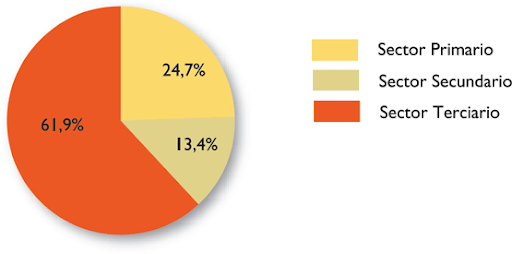
\includegraphics[scale = 0.35]{sectores}
			\centering
		\end{figure}
		\item \textbf{Diagrama de rectángulos o barras. }Consiste en varios rectángulos (uno por modalidad) de base constante y alturas proporcionales a las frecuencias (absolutas o relativas) de cada modalidad.
		\begin{figure}[h]
			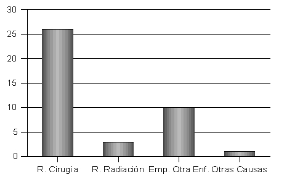
\includegraphics[scale = 0.5]{barras}
			\centering
		\end{figure}
	
		\item \textbf{Pictograma. }Se dibujan figuras, normalmente alusivas al carácter que se está estudiando, bien una para cada modalidad con tamaño proporcional a su frecuencia, o bien repitiendo la figura tantas veces como requieran las frecuencias.
		
		\begin{minipage}[t]{.45\linewidth}
		\raggedleft
		\vspace*{0pt}
		\begin{center}
			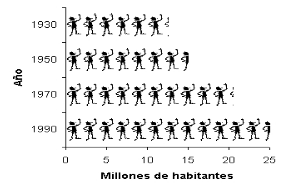
\includegraphics[scale = 0.5]{picto1}
		\end{center}
		\end{minipage}%
		\begin{minipage}[t]{.45\linewidth}
			\vspace*{0pt}
			\raggedleft
			\begin{center}
				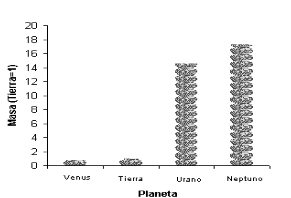
\includegraphics[scale = 0.5]{picto2}
			\end{center}
		\end{minipage}
	\end{itemize}
	
	\subsection{Variables discretas}
	
	\begin{itemize}
		\item \textbf{Diagrama de barras. }Sistema de ejes cartesianos en el que se representa en el eje de abcisas los valores de la variable, y se trazan barras verticales con longitudes proporcionales a sus frecuencias.
		\begin{minipage}[t]{.45\linewidth}
			\raggedleft
			\vspace*{0pt}
			\begin{center}
				\begin{tabular}{| c | c | c |}
					\hline
					$x_i$ & $n_i$ & $f_i = n_i / 100$ \\ \hline
					$0$ & $20$ & $0,2$ \\
					$1$ & $24$ & $0,24$ \\
					$2$ & $32$ & $0,32$ \\
					$3$ & $16$ & $0,16$ \\
					$4$ & $8$ & $0,08$ \\
					\hline
				\end{tabular}
			\end{center}
		\end{minipage}%
		\begin{minipage}[t]{.45\linewidth}
			\vspace*{0pt}
			\raggedleft
			\begin{center}
				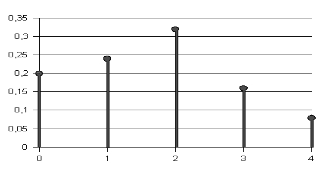
\includegraphics[scale = 0.5]{barra_discretas}
			\end{center}
		\end{minipage}
		\item \textbf{Curva de distribución}. Representación de la función de distribución, que es una función definida para cada número real $x$ como la proporción de datos menores o iguales que $x$. Así, si $x_1 < x_2 < \dots < x_k$ son los valores de la variable ordenados,
		
		\begin{minipage}[t]{.6\linewidth}
			\raggedleft
			\vspace*{0pt}
			\begin{equation*}
				F(x) = \left\{ \begin{array}{l}
					0 ~ \forall x < x_1\\
					\\ \dfrac{\sum_{j = 1}^i n_j}{n} = \sum_{j = 1}^i f_j = \dfrac{N_i}{n} = F_i ~ \forall x : x_i \leq x < x_{i+1} \\
					\\ 1 ~ \forall x \geq x_k
					\end{array}
				\right.
			\end{equation*}
			
		\end{minipage}%
		\begin{minipage}[t]{.45\linewidth}
			\vspace*{0pt}
			\raggedleft
			\begin{center}
				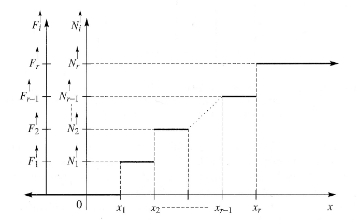
\includegraphics[scale = 0.5]{distrib_discreta}
			\end{center}
		\end{minipage}
	\end{itemize}
	
	\subsection{Variables continuas}
	
	\begin{itemize}
		\item \textbf{Histograma. }Está formado por rectángulos yuxtapuestos, cuyas bases son las diferentes clases o intervalos de definición de la variable, y cuyas alturas son las frecuencias medias $h_i = f_i/a_i$ por unidad de amplitud (densidades de frecuencia).
		
		\begin{minipage}[t]{.53\linewidth}
			\raggedleft
			\vspace*{0pt}
			\begin{center}
				\begin{tabular}{|r | c | c | c | c |}
					\hline
					$I_i$ & $n_i$ & $f_i$ & $h_i$ & Altura$_i = 5h_i$ \\ \hline
					$(0, 20]$ & $8$ & $8/70$ & $4/700$ & $2/70$ \\
					$(20, 30]$ & $9$ & $9/70$ & $9/700$ & $4.5/70$ \\
					$(30, 40]$ & $12$ & $12/70$ & $12/700$ & $6/70$ \\
					$(40, 45]$ & $10$ & $10/70$ & $10/700$ & $10/70$ \\
					$(45, 50]$ & $9$ & $9/70$ & $1.8/700$ & $9/70$ \\
					$(50, 60]$ & $10$ & $10/70$ & $10/700$ & $5/70$ \\
					$(60, 80]$ & $8$ & $8/70$ & $4/700$ & $2/70$ \\
					$(80, 100]$ & $4$ & $4/70$ & $2/700$ & $1/70$ \\
					\hline
				\end{tabular}
			\end{center}
			
		\end{minipage}%
		\begin{minipage}[t]{.45\linewidth}
			\vspace*{0pt}
			\raggedleft
			\begin{center}
				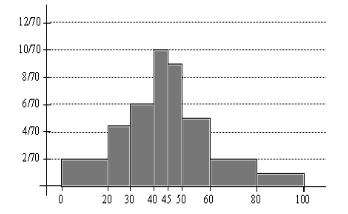
\includegraphics[scale=0.55]{histograma}
			\end{center}
		\end{minipage}
		\item \textbf{Poligonal de frecuencias. }Es la poligonal que resulta de unir los puntos correspondientes a los techos de las marcas de clase de los intervalos en el histograma.
		\begin{figure}[h]
			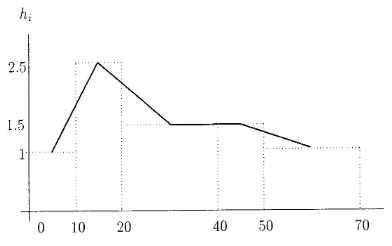
\includegraphics[scale=0.45]{poligonal_frec}
			\centering
		\end{figure}
	
		\item \textbf{Curva de distribución}.
		
		\begin{minipage}[t]{.45\linewidth}
			\raggedleft
			\vspace*{0pt}
			\begin{equation*}
				F(e_i) = \sum_{j = 1}^i f_j
			\end{equation*}
			\begin{equation*}
				F(-\infty) = 0, ~ F(+\infty) = 1
			\end{equation*}
		\end{minipage}%
		\begin{minipage}[t]{.45\linewidth}
			\vspace*{0pt}
			\raggedleft
			\begin{center}
				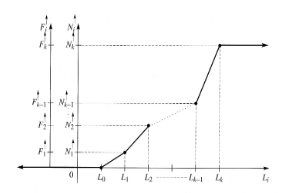
\includegraphics[scale=0.55]{distrib_continua}
			\end{center}
		\end{minipage}
	\end{itemize}

	\newpage

	\section{Características unidimensionales}
	
	Propiedades deseable (propiedades de Yule)
	\begin{enumerate}{}{}
		\item Deben definirse de manera objetiva, de forma que dos personas diferentes deben dar iguales resultados.
		\item Deben usar todas las observaciones y no algunas solamente.
		\item Deben tener un significado concreto, para que sean rápidas y fácilmente interpretables.
		\item Deben ser sencillas de calcular.
		\item Deben prestarse fácilmente al cálculo algebraico.
		\item Deben ser poco sensibles a fluctuaciones muestrales, de forma que si cambiasen valores extremos de los datos, no cambiasen en gran medida las características del conjunto.
	\end{enumerate}
	
	\subsection{Medidas de posición}
	
	\begin{itemize}
		\item \textbf{Media aritmética}. Es la suma de todos los valores de la variable dividida por el número total de observaciones.
		\begin{itemize}
			\item Si consideramos una variable estadística discreta en una población de tamaño $n$ con distribución ode frecuencias $\{(x_i, n_i(f_i)); i = 1, \dots, k\}$, la media aritmética es $$\overline{x} = \dfrac{1}{n} \sum_{i = 1}^k n_i x_i = \sum_{i = 1}^k f_i x_i$$
			\item Si la variable es continua y los datos están agrupados en intervalos de clase:
			$$\overline{x} = \dfrac{1}{n} \sum_{i = 1}^k n_i c_i = \sum_{i = 1}^k f_i c_i$$
			\item La media aritmética está acotada por los valores extremos de la variables: $x_1 \leq \overline{x} \leq x_k$.
			\item La media aritmética de las desviaciones de los datos respecto de la media aritmética es igual a cero: $$\sum_{i = 1}^k f_i (x_i - \overline{x}) = 0$$
			\item Si se somete una variable $X$ a una transformación lineal afín, la media aritmética de la nueva variable es la imagen de la media de $X$ por la misma transformación:
			$$Y = aX + b \Longrightarrow \overline{y} = a \overline{x} + b$$
			\item La media aritmética de los cuadrados de las desviaciones respecto a la media aritmética es mínima:
			$$\sum_{i = 1}^k f_i (x_i - \overline{x})^2 < \sum_{i = 1}^k f_i (x_i - a)^2, \qquad \forall a \neq \overline{x}$$
		\end{itemize}
	\item \textbf{Media geométrica}. Es la raíz $n$-ésima del producto de los $n$ valores (o marcas de clase) de la distribución: $$G = \sqrt[n]{\prod_{i=1}^{k} x_i ^ {n_i}}$$
	\item \textbf{Media armónica}. Se define como la inversa de la media aritmética de los valores inversos de la variable:
	$$H = \dfrac{n}{\frac{n_1}{x_1} + \frac{n_2}{x_2} + \cdots + \frac{n_k}{x_k}}$$
	\item \textbf{Media cuadrática}. Raíz cuadrada de la media aritmética de los cuadrados de los valores de la variables:
	$$Q = \sqrt{\sum_{i=1}^{k} f_i x_i^2}$$
	\item \textbf{Mediana}.
	\end{itemize}

	
\end{document}